\chapter{Migration von Sormas}

\section{SORMAS}
\label{ref:sormas_strucure}
Um die Anwendung \ac{SORMAS-ÖGD}(im weiteren zur Vereinfachung nur noch \ac{SORMAS}) erfolgreich migrieren zu können, müssen wir diese zunächst in ihre einzelnen Teile runterbrechen und identifizierne wofür die einzelnen Komponenten verantwortlich sind.
Da \ac{SORMAS} zum aktuellen Zeitpunkt als containerisierte Anwendung ausgerollt wird kann sich hier an der \textit{docker-compose.yaml}\footnote{https://github.com/hzi-braunschweig/SORMAS-Docker/blob/master/docker-compose.yml} orientiert werden.
Diese beschriebt 5 Container, die zusammen die Anwendung bilden.
\begin{itemize}
    \item sormas-application \\ Der Payara-Server auf dem die \ac{SORMAS}-Applikation gehostet wird.
    \item sormas-postgres \\ Die Datenbank in der die Daten aus der Anwendung gespeichert werden.
    \item sormas-pg-dump \\ Dieser Container ist ausschließlich dafür verantwortlich in bestimmten Zeitabständen einen Datenbankdump der Postgres-Datenbank zu machen.
    \item sormas-apache2 \\ Der Webserver ist für die Terminierung der \ac{SSL}-Zertifikate Froggo
    \item autoheal \\ Damit können gestoppte oder ungesunde Container neu gestartet werden
\end{itemize}
Da die Anwendung nach Kubernetes migriert werden soll, können einige der Funktionen von den Kubernetes-eigenen Funktionalitäten übernommen werden. 
Der Ingress kann die Terminierung der \ac{SSL} Zertifikate managen und wird den Apache Webserver ersetzen.
Die Autoheal Funktion gehört zu den Grundfunktionen von Kubernetes und muss nicht extra implementiert werden, wenn die Anwendung als ReplicaSet oder Deployment ausgerollt wird.
Der Container, der nur die Datenbank Dumps ausführt, kann durch einen Cronjob abgebildet werden. 
Die einzigen Container die dann noch übernommen werden sind der Payara-Server und die PostgreSQL-Datenbank.
Zusätzlich müssen Ingress und Cronjob konfiguriert werden. \\
Doch zunächst sollen einzelne Funktionen von Kata getestet werden.


\section{Erste Tests mit der Kata Runtime}
Noch bevor begonnen wurde das Cluster aufzubauen, wurden erste Test mit der Kata-Runtime durchgeführt. 
Mit diesen wurde überprüft ob schon im voraus Probleme identifiziert werden konnten, die die Umsetzung verhindern würden. 

\subsection{Docker Kata Integration}
Als erstes wurde ein Container in der Kata Runtime über die bereits installiert Container Engine Docker gestartet.
Mit dem Command \texttt{uname -a} kann der in dem Container verwendete Kernel ausgegeben werden. 
Wenn man diesen mit dem Kernel des Host Systems vergleicht lässt sich feststellen ob beide auf dem gleich Kernel laufen, wie es bei Docker containern der FAll wäre, oder ob ein eigener Kernel für die VM virtualisiert wurde.
\\
Über Docker lassen sich Kata-Container mit der \texttt{--runtime=kata} starten.
Als Images wurden kleine Alpine-Container gewählt.
Um einen Vergleich zwischen beiden Runtimes zeihen zu können wurde ein kurzen Skript gechrieben, dass die Startup-Zeiten in eine Datei schreibt.
Das Skript unter \ref{lst:startuptimes} ergab auf meiner Maschine eine zeitliche Differenz von ca. einer Sekunde wie aus \ref{app:startuptimecomparison} zu entnehmen ist. 
Die wichtigste Erkenntnis an dieser Stelle ist jedoch, dass die Container in der neuen Runtime problemlos starten, und dazu tatsächlich einen anderen Kernel gestartet bekommen.

\begin{lstlisting}[language=bash, caption={compare\_startup\_times.sh}, label=lst:startuptimes]
#!/bin/bash
touch startuptime_comparison
echo runc: > startuptime_comparison
{ time docker run --rm --runtime=runc archlinux sh -c 'uname -r'; } 2>> startuptime_comparison
echo kata-runtime: >> startuptime_comparison
{ time docker run --rm --runtime=kata archlinux sh -c 'uname -r'; } 2>> startuptime_comparison
\end{lstlisting}

\subsection{Webapp in Kata}
Im nächsten Test soll das Deployment einer Web-Anwendung in Kata gestestet werden. 
Dafür habe ich das Docker-Image eiener Website zum Thema der Web\ac{API}s verwendet, das während des letzten Semesters erstellt wurde, gewählt. 
Tatsächlich mussten hier gar keine Anpassungen oder Ähnliches vorgenommen werden. 
Die \texttt{runtime}-Flag wurde gesetzt und beim Start konnte der andere Kernel nachgewiesen werden.
Ansonsten ließen sich keine Änderungen in dem Verhalten der Anwendung feststellen. 
Das Austauschen der Runtime verlief komplett nach dem von Kata Angestrebten Plug-and-Play Prinzip.
Hier wurden die Möglichkeiten, die durch das einheitliche Verwenden der Schnittstellen ermöglicht werden, deutlich. 

\subsection{PostgreSQl in Kata}
Als letzter grundlegender Test sollte eine PostgreSQL Anwendung in der Kata-Runtime deployed werden. 
Dabei wurden aufgrund der simplen Migration der Webapp keine größeren Probleme erwartet.
Doch an dieser Stelle machten sich zum ersten Mal Probleme mit der Kata-Runtime bemerkbar.
\\
Das Starten der Anwendung war noch sehr uproblemantisch, alle bnötigten Variablen konnten über eine enviroments-Datei übertragen werden und die Runtime wie zuvor über die entsprechende Flag definiert werden. 
Wurde der Container nach dem Start der Anwendung jedoch betreten und man versucht von dort aus in die Postgres Datenbank zu kommen, erhielt man folgenden Fehler:
\\\texttt{could not connect to server, temporary failure in name resolution}\\
Die Datenbank ist allerdings von außerhalb erreichbar, wurde kein \texttt{docker exec} in den Container ausgeführt, sondern direkt von der Host-Maschine aus der ZUgriff auf die Datenbank gestartet, konnte diese ohne Probleme bedient und gemanaged werden. 
Das Problem ließ sich zwar in der dafür aufgebrachten Zeit nicht lösen, da die Datenbank aber trotzdem erreicht wurden konnte sollte diese Einschränkung kein Problme darstellen. 

Die grundlegenden Tests können damit als abgeschlossen betrachtet werden und es kann mit dem nächsten Schritt, dem Übersetzen der docker-compose Datei zu Kubernetes Manifesten, begonnen werden. 
Zunächst muss dieser Schritt getan werden, damit anschließend die Runtime auf Kata umgestellt und dann gedebugged werden kann. 


\section{Migration der Anwendung nach Kubernetes}

\subsection{Struktur}
Als erstes wurde die Struktur der Kubernetes Anwendung geplant. 
Die schon in Absatz \ref{ref:sormas_strucure} festgehalten, können einige Container ignoriert werden, da Ihre Funktion standartmäßig in Kubernetes integriert ist. 
Die restlichen Container müssen jedoch zu Deployments oder StatefulStes übersetzt werden, mit Services zugänglich gemacht, und mit Secrets sowie ConfigMaps konfiguriert. 
Außerdem müssen den Anwendunge \ac{PV}s zugeordnet werden und sie müssen mittels eines Ingresses erreichbar gemacht werden.
Der genaue Aufbau wurde in Abildung \ref{fig:sormas_kubernetes} dargestellt. 
Aus Gründen der Überscihtlichkeit wurde hierbei auf die Darstellung der Backup-Funktionalitäten verzichtet, diese werden später genauer erklärt.

\begin{figure}[h!]
\centering    
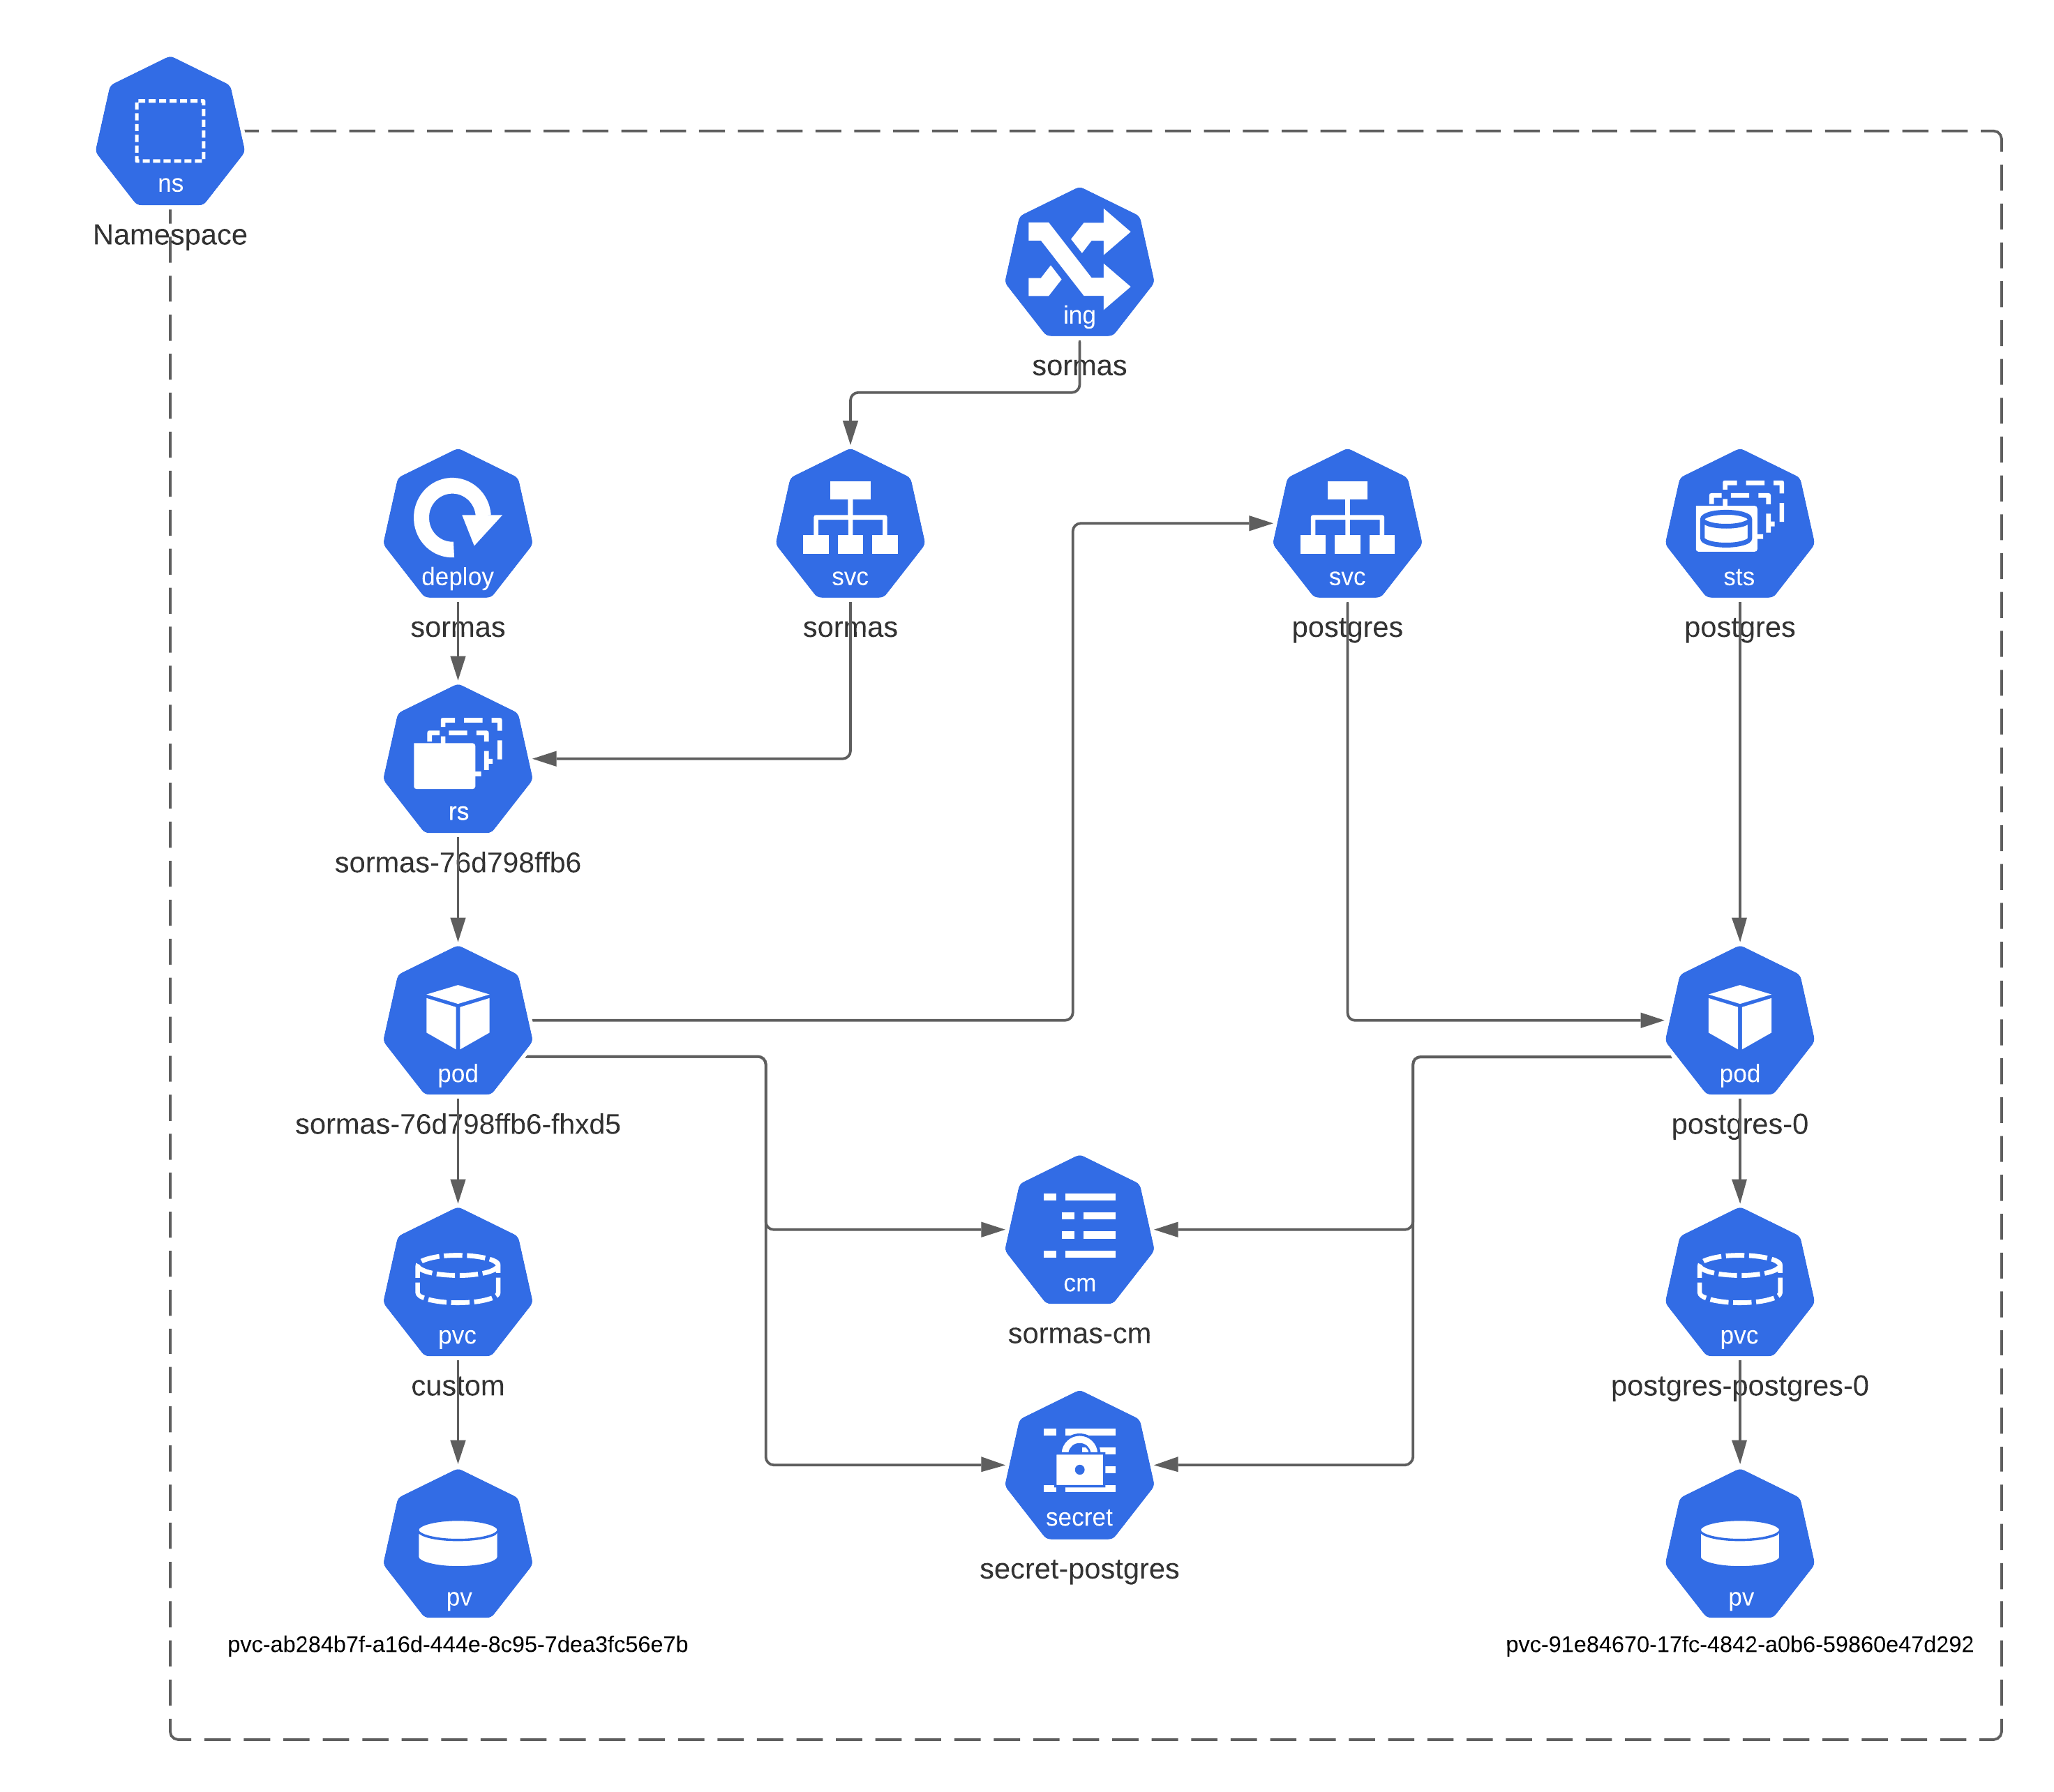
\includegraphics[width=\textwidth]{bilder/sormas_kubernetes.png}
\caption{SORMAS in Kubernetes}
\label{fig:sormas_kubernetes}
\end{figure}

Als Element zur Trennung und Organisation der einzelnen \ac{SORMAS}-Instanzen wird für jedes \ac{GA} ein eigener Namespace angelegt.
So kann jeder Pod genau einem \ac{GA} zugeordnet werden.\\
Wie zuvor angemerkt, ersetzt der Ingress an dieser Stelle den zuvor zur \ac{SSL}-Terminierung benötigten Apache2 Webserver.\\
Die Datenbank wird in einem StatefulSet ausgerollt, da diese durch die genaue Bestimmung der Pods besser persistent gestaltet werden kann.
Das StatefulSet erstellt dann seinen benötigten Pod, der über ein \ac{PVC} sein \ac{PV} zugeordnet bekommt. 
Die Konfiguration des Pods soll ausschließlich in der ConfigMap und dem Secret stattfinden, sodass nur an einer Stelle Anpassungen vorgenommen werden müssen.
Der Pod kann durch das Einrichtigen eins Services für andere Instanzen im selben Namespace erreichbar gemacht werden.\\
Der Payara-Server wird mit einem Deployment-Manifest ausgerollt. 
Die Eigenschaften des StatefulSets werden nicht benötigt und die Vorteile in Hinsicht auf das erleichterte Updaten der Software werden für zu erwartende Updates nützlich sein.
Das Deployment erstellt dann das entsprechende ReplicaSet und dieses den Pod. 
\ac{PV} und Konfiguration werden analog zu Postgres gemanaged. 
Der Service wählt mittels des Selectors allerdings das ReplicaSet und nicht den Pod selbst.


\subsection{Schreiben der Kubernetes Manifeste}

Alle geschriebenen Manifeste, auch die auf die in diesem Abschnitt nicht weiter eingegangen wird, sind auf Github veröffentlicht und können dort unter \url{https://github.com/robbmue/katanetes_sormas/tree/master/manifests} eingesehen werden. 

Beim Schreiben der Manifeste diente die \textit{docker-compose.yml}\footnote{https://github.com/hzi-braunschweig/SORMAS-Docker/blob/master/docker-compose.yml} als Vorlage.
Aus dieser wurden zunächst einmal alle Services eliminiert die in Kubernets nicht weiter benötigt werden, namentlich den Autoheal, den Apache2 Webserver und den pg-dump.
Die beiden letzen Teile der Anwendung wurden dann entsprechend der vorhergehenden Planung in jeweils ein Deployment und ein StatefulSet übersetzt.
Zuerst wurde ein Namespace für die komplette Anwendung angelegt, in dem alle restlichen Teile deployed werden.

\hfill \newline
\subsubsection{Payara Deployment}
Bei dem Payara Server ist vor allem wichtig, deren speziellen Port in das Manifest miteinzubinden.
Payara nutzt als Standart-Port 6080 und als Admin-Port 6048, diese werden unter den Namen \texttt{payara} und \texttt{payara-admin} dem Deployment hinzugefügt.
Abhängig von diesen ist auch die liveness- und readinessProbe, hier werden diese mit einem \ac{HTTP}-GET auf den entsprechenden Port und den \ac{SORMAS}-Pfad \texttt{/sormas-ui/login} realisiert.
Wenn diese Seite erreichbar ist, kann von einer funktionierenden Instanz ausgegangen werden.
Der Service, der auf diese Anwendung verweist, wird so konfiguriert, dass dieser auf Port 80 lauscht aber alle eingehenden Anfragen an Port 6080 des Payara-Pods weiterleitet.
So kann der ungewöhnliche Port des Payara-Servers in einen Standart-Port umgewandelt werden. 
Der Ingress wiederum zeigt auf den Service und Sorgt dafür, dass die Anwendung von außerhalb erreichbar ist.

Des weiteren muss das \ac{PV} mittels des \ac{PVC} eingebunden werden und die Enviroment-Variablen müssen gesetzt werden. 
Der \ac{PVC} wird unter dem Punkt \texttt{volumes} dem Pod zugewiesen und unter \texttt{volumeMounts} wird der Pfad angegeben, an der das Volume eingahngen werden soll. 
Die Variablen setzt man unter dem Punkt \texttt{env}, hier kann sowohl auf ein Secret, als auch auf eine ConfigMap zugegriffen werden und diese zu setzen.
Es könnten auch direkt in dem Deployment die korrekten Werte gesetzt werden, mit der ConfigMap und dem Secret wird jedoch erreicht, dass Änderungen nur an möglichst wenigen Stellen vorgenommen werden müssen.
Außerdem wird auch das StatefulSet auf die gleichen Dateien zugreifen, und so kann garantiert werden, dass beide Anwendungen übereinstimmende Werte geliefert bekommen.

Zuletzt werden noch Limits für \ac{CPU} und Memory-Nutzung gesetzt. 

Auf die Manifeste für den \ac{PVC}, die ConfigMap und das Secret soll hier nicht weiter eingegangen werden da diese keine Großen Besonderheiten enthalten. 

\hfill \newline
\subsubsection{SORMAS StatefulSet}
Für die Datenbank wurden Konfigurationen analog zu denen des Payara-Servers vorgenommen.
Der Port 5432 wurde freigegeben, die Enviroment Variablen und der \ac{PVC} wurden eingebunden sowie limits gesetzt.
Eine Besonderheit in diesem Manifest ist, dass mit dem \texttt{args} Parameter gearbeitet werden muss. 
Es muss eine Änderung an dem Parameter \texttt{max\_prepared\_connections} in der \textit{postgresql.conf} vorgenommen werden, damit \ac{SORMAS} starten kann. 
Der Postgres Container startet immer mit dem \texttt{psql} Kommando, also kann mittels des Arguments \texttt{-c config\_file=/etc/postgresql/postgresql.conf} die Config eingelesen werden.

Auf den Service und den \ac{PVC} soll an dieser Stelle nicht weiter eingegangen werden, sie können auf Github nachgelesen werden. 


\hfill \newline
\subsubsection{Backup}
Als Backup-Lösung wurde Stash\footnote{https://stash.run/\#} von AppsCode\footnote{https://appscode.com/} gewählt.
Die Software erlaubt es unter anderem Backups auf einem lokalen Storage zu erstellen und mit Datenbankdumps zu arbeiten, nicht nur mit Volume Snapshots.

Bei Netzlink wird ein lokaler Minio\footnote{https://min.io/} \ac{S3}-Storage gehostet, in dem die Backups gespeichert werden können.
Damit Stash die Verbindung zu diesem aufbauen kann muss zunächst ein Secret erstellt werden, dass die Anmeldedaten für den \ac{S3} Storage beinhaltet.
Aufbauend darauf kann dann die \ac{CRD} \texttt{Repository} deployed werden. 
Diese gibt die Addresse des \ac{S3} Storages an, sowie den Bucket in den gespeichert werden soll und das zur Organisation verwendete Prefix.
Außerdem beinhaltet die Repository-Ressource auch das zuvor definierte Secret und bindet dieses so an das Repository.
\\
Als nächstes wird die \ac{CRD} \texttt{AppBinding} erstellt. 
Über dieses AppBinding wird benötigt um auf die Datenbank zuzugreifen. 
Dazu braucht es den Service und Port, sowie das Schema und den Typen der Datenbank und letzten endes ein Secret, aus dem der Datenbanknutzer und sein Password ausgelesen werden können.
In dieser einen \ac{CRD} sind dann also alle Informationen gesammelt um auf die Datenbank zuzugreifen und in dem Repository ist definiert wohin das Backup gespeichert werden soll.
Als letztes fehlt also nur noch eine Ressource, die das Backup anstößt.
\\
Diese \ac{CRD} nennt sich \texttt{BackupConfiguration}. 
In ihr wird 
\begin{itemize}
    \item das \texttt{AppBinding} und das \texttt{Repository} zusammengetragen
    \item der auszuführende Task angegeben (in dem Version und Art der Datenbank festgelegt sind)
    \item eine \texttt{retentionPolicy} definiert (diese gibt an wie viele der erstellten Backups erhalten bleiben sollen)
    \item der \texttt{schedule} in CronJob Syntax angegeben
\end{itemize}
Stash erzeugt aus diesen \ac{CRD}s dann Ressourcen, mit denen Kubernetes arbeiten kann.
Alle benötigten Informationen werden in einem Kubernetes nativen CronJob zusammengetragen.
Ein CronJob in Kubernets erstellt sich immer zur definierten Zeit einen Job. 
Ein Job wiederum erstellt einen oder mehrere Container, die nur eine genau abgegrenzte Aufgabe haben, und stellt sicher dass diese erfolgreich terminieren. 
In diesem Fall ist die Aufgabe das Erstellen das Datenbankdumps, das Verschlüsseln und Kopieren der verschlüsselten Daten auf den \ac{S3} Storage plus das Löschen der überschüssigen, bereits vorhandenen Datenbankdumps.
Nach der erfolgreichen Ausführung all dieser Operationen terminiert der Job und alle Pods werden gestoppt. 
So kann garantiert werden, dass das Backup nur während der Ausführung Compute-Ressourcen verbraucht. 


\section{Migration der Anwendung zur Kata-Runtime}


\subsection{Migration des Payara Servers}


\subsection{Migration der PostgreSQl-Datenbank}


\section{Helm Templating}